% tikzpic.tex
\documentclass[crop,tikz]{standalone}% 'crop' is the default for v1.0, before it was 'preview'

\usetikzlibrary{arrows,decorations.pathmorphing,decorations.pathreplacing,backgrounds,positioning,fit,matrix}
\usetikzlibrary{shapes,calc,patterns,arrows.meta}
\tikzset{
	vert/.style={circle,inner sep=1.5,fill=white,draw,minimum size=.3cm},
	edge/.style={color=black, thick},
	diredge/.style={->,>={Stealth[width=8pt,length=8pt]},color=black, thick},
	timelabel/.style={fill=white,font=\footnotesize, text centered},
	wave/.style={decorate,decoration={coil,aspect=0}},
	dirwave/.style={->, >={Stealth[width=8pt,length=8pt]},decorate,decoration={coil,aspect=0}},
	diredge2/.style={->,>={Stealth[width=8pt,length=8pt]}}
}
\begin{document}
	
	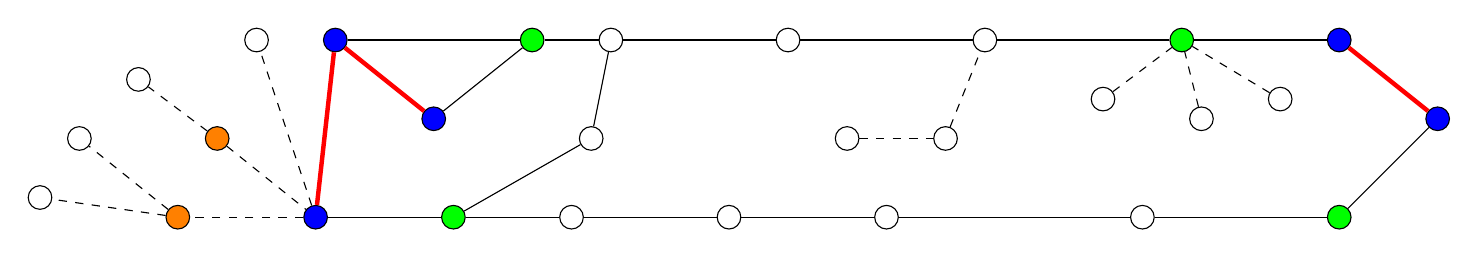
\begin{tikzpicture}
		\node [vert, fill = blue] (0) at (-14, 0) {};
		\node [vert, fill = green] (1) at (-12.25, 0) {};
		\node [vert, fill = white] (2) at (-10.75, 0) {};
		\node [vert, fill = white] (3) at (-8.75, 0) {};
		\node [vert, fill = white] (4) at (-6.75, 0) {};
		\node [vert, fill = white] (5) at (-3.5, 0) {};
		\node [vert, fill = green] (6) at (-1, 0) {};
		\node [vert, fill = blue] (7) at (0.25, 1.25) {};
		\node [vert, fill = blue] (8) at (-1, 2.25) {};
		\node [vert, fill = green] (9) at (-3, 2.25) {};
		\node [vert, fill = white] (10) at (-5.5, 2.25) {};
		\node [vert, fill = white] (11) at (-8, 2.25) {};
		\node [vert, fill = white] (12) at (-10.25, 2.25) {};
		\node [vert, fill = white] (14) at (-1.75, 1.5) {};
		\node [vert, fill = white] (15) at (-4, 1.5) {};
		\node [vert, fill = white] (16) at (-6, 1) {};
		\node [vert, fill = white] (17) at (-7.25, 1) {};
		\node [vert, fill = blue] (18) at (-13.75, 2.25) {};
		\node [vert, fill = blue] (19) at (-12.5, 1.25) {};
		\node [vert, fill = green] (20) at (-11.25, 2.25) {};
		\node [vert, fill = orange] (21) at (-15.25, 1) {};
		\node [vert, fill = white] (22) at (-16.25, 1.75) {};
		\node [vert, fill = white] (23) at (-17, 1) {};
		\node [vert, fill = orange] (24) at (-15.75, 0) {};
		\node [vert, fill = white] (25) at (-17.5, 0.25) {};
		\node [vert, fill = white] (26) at (-2.75, 1.25) {};
		\node [vert, fill = white] (27) at (-10.5, 1) {};
		\node [vert, fill = white] (28) at (-14.75, 2.25) {};
		
		
		\draw (1) to (2);
		\draw (2) to (3);
		\draw (3) to (4);
		\draw (4) to (5);
		\draw (5) to (6);
		\draw (6) to (7);
		\draw (8) to (9);
		\draw (9) to (10);
		\draw (10) to (11);
		\draw (11) to (12);
		\draw (20) to (12);
		\draw (19) to (20);
		\draw [dashed] (0) to (24);
		\draw [dashed] (24) to (25);
		\draw [dashed] (24) to (23);
		\draw [dashed] (21) to (0);
		\draw [dashed] (21) to (22);
		\draw [dashed] (16) to (10);
		\draw [dashed] (17) to (16);
		\draw [dashed] (14) to (9);
		\draw [dashed] (15) to (9);
		\draw [dashed] (26) to (9);
		\draw (27) to (12);
		\draw (27) to (1);
		\draw (18) to (20);
		\draw [dashed] (0) to (28);
		\draw (0) to (1);
		\draw [ultra thick, red] (8) to (7);
		\draw [ultra thick, red] (18) to (0);
		\draw [ultra thick, red] (19) to (18);
		
	\end{tikzpicture}
	
	
\end{document}